\chapter{はじめに}

\section{研究背景}
本研究の背景には,ニューラルネットワークを用いた深層学習と格子ボルツマン法(Lattice Boltzmann Method, LBM)の二つの重要な要素がある.一方の深層学習は機械学習の一分野であり,複数の隠れ層を持つニューラルネットワークを使って複雑なパターンを学習する手法である.近年盛んに研究されていて応用先の一つに気象予測があり\cite{Schultz2021},例えばCNNとLSTMを用いた正方形領域での風速予測がされている\cite{CHEN2021114451}.他方で,格子ボルツマン法は比較的新しい数値流体力学の手法であり,個々の粒子のふるまいを扱うのではなく,格子状に分割した空間内で各格子点上の離散化された速度分布関数を解くものである\cite{doi:10.1146/annurev.fluid.30.1.329}.この手法の長所として並列計算と相性がよいことが挙げられ,GPUやTPUのようなプロセッサ上で効率的に計算することができる\cite{Satofuka1999}.これはニューラルネットワークにも共通する特性である.

\section{先行研究}
\subsection{CNNとLSTMを用いた正方形領域での風速予測 \label{subsec:chen2021}}
Chenら(2021)は,CNNとLSTMを用いた正方形領域での風速予測を行った\cite{CHEN2021114451}.彼らのモデル概要図を図\ref{fig:chen2021_architecture}に示す.この図において,エンコーダとデコーダの部分にCNNが用いられており,これにより正方形領域における格子点上の風速の空間的なパターンを学習している.また,エンコーダの出力をLSTMに入力し,更にその出力をデコーダに入力している.このLSTMのユニットにより,時間的なパターンも学習している.
\begin{figure}[tbp]
    \centering
    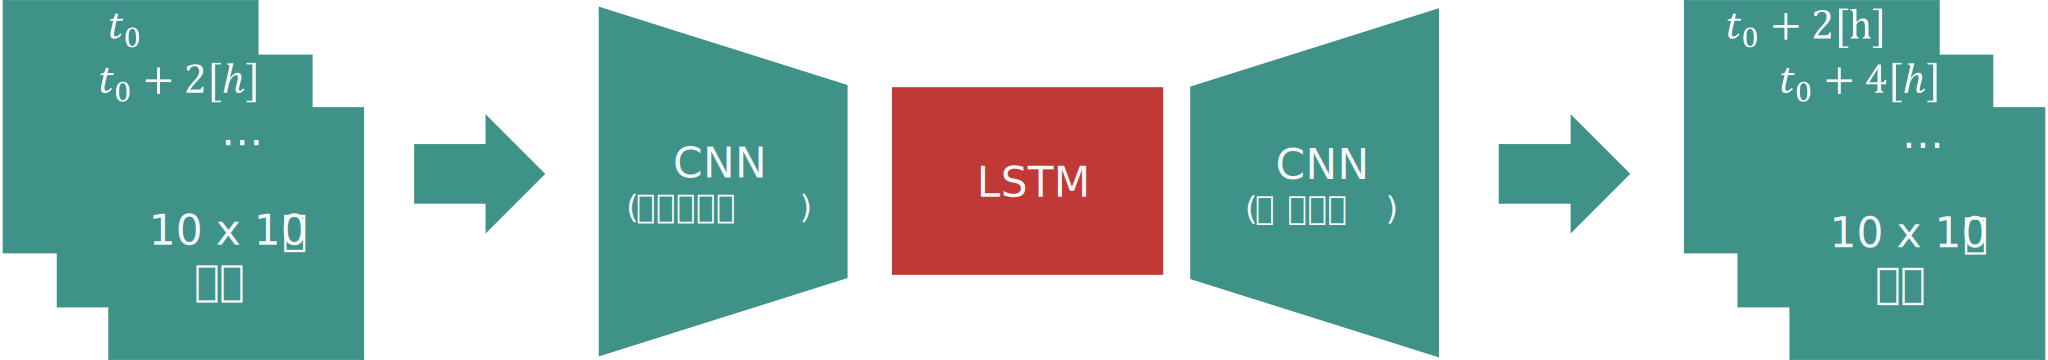
\includegraphics[width=0.9\textwidth]{./introduction/figs/chen2021_model_overview.svg.eps}
    \caption{Chenら(2021)のモデル概要図\cite{CHEN2021114451}}
    \label{fig:chen2021_architecture}
\end{figure}

このモデルを使って,彼らは図\ref{fig:chen2021_region}に示すようにアメリカのインディアナ州内部で,2km間隔の$10 \times 10$格子点上で2時間先の風速予測を行い,単にANNやLSTMのみを用いたモデルに比較して精度が向上することを示した.具体的には,全体の風速予測の平均絶対誤差(Mean Absolute Error, MAE)が$0.35 \mathrm{m/s}$減少し,これはpersistanceなモデル,ANNのみのモデル, LSTMのみのモデルの結果に比べてそれぞれ$32.7\%$, $28.8\%$, $18.9\%$低い値であると主張している.ここで,persistanceなモデルとは,風速の時間変化を考慮せず,直前の風速をそのまま予測値とするモデルである.
\begin{figure}[tbp]
    \centering
    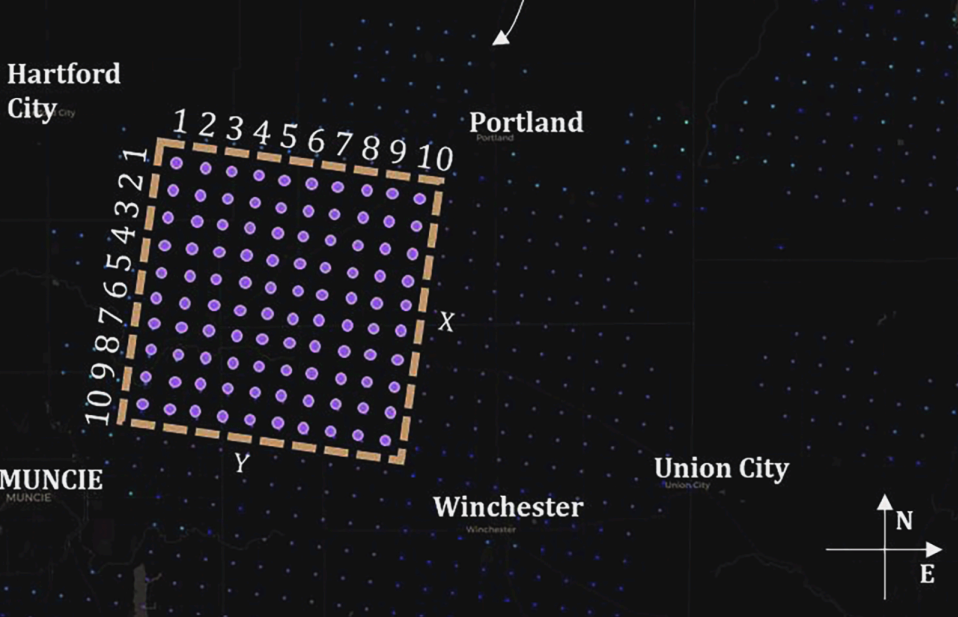
\includegraphics[width=0.8\textwidth]{./introduction/figs/chen2021_region.png.eps}
    \caption{Chenら(2021)が風速予測を行った範囲\cite{CHEN2021114451}}
    \label{fig:chen2021_region}
\end{figure}


\if 0
PINNのやつをいれて,これは大気のシュミレーションには向いていない,なぜなら拘束条件が不明だから
みたいなことをかく
\fi

\subsection{}

\section{研究目的}
本研究では\ref{subsec:chen2021}節で述べたChenら(2021)の研究と同様に,長方形領域における格子点上での風速予測を行うが,ニューラルネットワークの構造にLBMを組み込むことで,LBMの持つ並列計算と相性の良さを活かしつつ,精度の向上を図る.
% todo: 結果とか考察を加味して後で加筆修正,その際に修論概要書と整合性をとる

\section{論文構成}
TBD 